%\typeout{IJCAI-16 Instructions for Authors}
\documentclass{article}
\usepackage{ijcai16}
% Use the postscript times font!
\usepackage{times}
% the following package is optional:
%\usepackage{latexsym}
\usepackage{amssymb}
\usepackage{amsmath}
\usepackage[disable]
{todonotes}
\usepackage{siunitx}

% TODO length of the paper: 6 pages + 1 page for references
% TODO grayscale figures
\title{
Accelerating Refinement of Demonstrated Skills in Task Space with
Approximate Inverse Kinematics}
% Commented for blind review
\author{Alexander Fabisch \and Manuel Meder
\thanks{
This work was supported through two grants of the German Federal Ministry of
Economics and Technology (BMWi, FKZ 50 RA 1216 and FKZ 50 RA 1217).}\\
Robotics Research Group, University of Bremen\\
alexander.fabisch@dfki.de \and manuel.meder@dfki.de}
%\author{
%learning from demonstration,
%imitation learning,
%reinforcement learning,
%policy search,
%inverse kinematics}

\begin{document}

\maketitle

\begin{abstract}
Transfering skills between different kinematic structures
(for example from a human or another robot to a robotic target system)
is straightforward in Cartesian space.
Because of the correspondence problem, however, the result will most likely
not be identical.
This is why refinement is required afterwards, for example,
by reinforcement learning. Reinforcement learning %with state-of-the-art methods
in Cartesian space is prone to reachability problems when using conventional
inverse kinematic solvers. We propose a configurable approximate inverse
kinematics solution and show that it accelerates the refinement process
considerably.
In addition, we conduct a thorough empirical comparison refinement in task
space and refinement in joint space.
\todo[inline]{Update abstract}
\end{abstract}

\section{Introduction}

In order to create autonomous robotic systems in real, dynamic environments
machine learning approaches for robotic skills are required.
Skill learning frameworks for robots often combine various approaches to
leverage intuitive knowledge from humans \cite{Peters2012,Metzen2013}.
\todo[inline]{Replace citation by Frontiers paper?}
Most of these fall into the two categories imitation learning and reinforcement
learning. A standard approach to learning skills is to initialize with
a demonstrated movement and then refine the skill with policy search
\cite{Kober2012,Deisenroth2013}.
Both methods are complementary because on the one hand policy search methods
are often local search approaches that require good initialization and
on the other hand imitation learning usually does not produce a perfect
skill from the start because of the correspondence problem \cite{Argall2009},
that is, different kinematic and dynamic properties of the target system and
the demonstrator result in different outcomes.

We think that it is sometimes better to do policy search directly in task
space because demonstration and main objectives of the learning problem are
given in task space.
However, when policy search methods are used to learn end-effector
trajectories in task space, it often occurs that a trajectory is not
completely in the robot's workspace or a requested orientation cannot
be reached exactly. This results in a reward landscape with flat regions
or abrupt changes.

\section{Related Work}

In this section, we will present the setting in which our problem is embedded
and then give a brief overview of the current state of the art in inverse
kinematics that is related to our work.

\subsection{Transfering Skills in Task Space}

% http://www.cs.cmu.edu/~mmv/papers/09ras-survey.pdf \cite{Argall2009}
Transfering skills from humans to robots without kinesthetic teaching
is prone to the correspondence problem. Especially relevant for our work
is the embodiment mapping \cite{Argall2009}. Consider for example a
reaching trajectory that is recorded from a human and transfered to the
robot's end-effector. Because the robot probably has a different hand shape,
it cannot grasp the object with exactly the same end-effector trajectory.
In this case, policy search in Cartesian space can be used used to refine the
initial trajectory.
Transfering trajectories directly in joint space is even more difficult
because the segment lengths of a robot arm and the human arm are most likely
very different.

Examples for skills that have been demonstrated in task space and transfered
to robots are pancake flipping (demonstration by kinesthetic teaching;
\cite{Kormushev2010}), peg in hole (demonstration by tele-operation;
\cite{Krueger2014}), and water-serving (demonstration by kinesthetic
teaching of a similar arm \cite{Pastor2009}).
There are several reasons why we should often learn trajectories in task space.
Learning in Cartesian space is often easier when the main objectives are
defined in Cartesian space. For example, learning in joint space when we want
to grasp an object might result in too complex Cartesian trajectories.
When we want to transfer a skill from one robot to another it is easier to
go over the end-effector pose instead of joint angles because of different
kinematic structures \cite{Pastor2009}. This way, half of the embodiment
mapping is done by forward and inverse kinematics.
%it is easier to optimize the trajectory there \cite{Kormushev2010},
%to accelerate transfer to new task configurations \cite{Krueger2014}
% maybe as an example for generalization in task space:
% https://ewrl.files.wordpress.com/2011/08/ewrl2011_submission_30.pdf
% http://kormushev.com/papers/Kormushev-IROS2010.pdf \cite{Kormushev2010}
% http://citeseerx.ist.psu.edu/viewdoc/download?doi=10.1.1.152.2383&rep=rep1&type=pdf \cite{Pastor2009}

All of the mentioned works use
dynamic movement primitives (DMP) as underlying trajectory representation.
In our work, we will use a DMP based on quaternions \cite{Ude2014}
to represent end-effector orientations and another variant \cite{Muelling2013}
to represent positions.

\subsection{Inverse Kinematics}

Let $\boldsymbol{q}_t$ be the joint angles of a kinematic chain at time $t$.
The forward kinematics of the chain is given by
$$f(\boldsymbol{q}_t) = \boldsymbol{p}_t,$$
where $\boldsymbol{p}_t$ denotes the end-effector's pose in Cartesian space
consisting of the position and rotation.
An exact solution to the inverse kinematics problem would represent
$$f^{-1}(\boldsymbol{p}_t) = \boldsymbol{q}_t.$$
However, $f^{-1}$ is usually not a function. Many joint configurations might
result in the same end-effector pose.
In addition, often it is not possible to find an exact solution to the problem.

Numerical inverse kinematics approaches are an efficient way to deal with
redundant kinematic chains that might have many solutions or very complex
analytical solutions.
Widely used classical approaches are often based on the Jacobian pseudo-inverse
or Jacobian transpose \cite{Nilsson2009}. However, sequential quadratic
programming has been shown to outperform these methods in terms of
joint limit handling and and computation time \cite{Beeson2015}.
It has already been shown by Beeson~and~Ames~\shortcite{Beeson2015} that
indirect inverse kinematics formulations of the form
\begin{eqnarray*}
\arg\min_{\boldsymbol{q}_t \in \mathbb{R}^n}&&
  (\boldsymbol{q}_{t-1} - \boldsymbol{q}_t)^T (\boldsymbol{q}_{t-1} - \boldsymbol{q}_t)\\
\text{s.t.} &&
  g_i(\boldsymbol{q}_t) \leq b_i, \quad i = 1, \ldots, m
\end{eqnarray*}
where the constraints include the Euclidean distance error, the angular
distance error, and joint limits (e.g. \cite{Kumar2010,Fallon2015}), have a
much lower success rate than direct formulations of the form
\begin{eqnarray}
\label{ikproblem1}
\arg\min_{\boldsymbol{q}_t \in \mathbb{R}^n}&&
%  d(f(\boldsymbol{q}_t) \cdot f(\boldsymbol{q}_t))\\
  d(f(\boldsymbol{q}_t), \boldsymbol{p}^{\text{des}}_t))\\
\label{ikproblem2}
s.t. &&
  g_i(\boldsymbol{q}_t) \leq b_i, \quad i = 1, \ldots, m
\end{eqnarray}
where $d$ is a pose distance metric, $\boldsymbol{p}^{\text{des}}_t$
is the desired end-effector pose, and the inequality constraints only
consist of the joint limits. Several distance metrics are compared by
Beeson~and~Ames~\shortcite{Beeson2015}.

Few works investigate approximate inverse kinematics solutions.
However, in cases where the desired end-effector pose cannot be reached
exactly, we would like to have at least the closest possible solution.
Unreachable poses might be a problem of robots that have a low number of
joints \cite{Henning2014} or at the borders of workspaces as this can be
seen for example in visualizations of capability maps \cite{Zacharias2007}.
Traditional methods based on the Jacobian pseudoinverse tend to be
instable and run into local minima \cite{Nilsson2009,Henning2014}.
Henning~\shortcite{Henning2014} investigated an approximate inverse
kinematic based on a database motivated amongst others by
the work of Satzinger~et.~al~\shortcite{Satzinger2014}.

\section{Configurable Approximate Inverse Kinematics}

A disadvantage of previous approaches is that they do not allow to
configure the approximation.
In the domain of robot skill learning it is often not required to reach
each requested pose in a trajectory exactly. In particular, it is often
not required to reach each orientation perfectly.
Consider for example the problem of learning to grasp an object. At the
beginning of a reaching movement it is not relevant how the end-effector
is rotated. It only becomes important at the end of the movement.
That is the reason why we develop a more relaxed objective for our
inverse kinematic solver based on the work of
Beeson~and~Ames~\shortcite{Beeson2015}.

Starting from the inverse kinematics formulation in Equations
\ref{ikproblem1} and \ref{ikproblem2}, we can replace the pose distance metric
by a weighted version of the form
\begin{eqnarray*}
d(\boldsymbol{p}_1, \boldsymbol{p}_2) &=&
  w_{\text{pos}}||\boldsymbol{p}_{1, 1:3} - \boldsymbol{p}_{2, 1:3}||_2^2\\
&&
  + w_{\text{rot}} \left[ 2 \arccos\left(\boldsymbol{p}_{1, 3:7} \cdot \overline{\boldsymbol{p}}_{2, 3:7}\right)\right]^2,
\end{eqnarray*}
where $\boldsymbol{p}_{1:3}$ represents the position of the end-effector and
$\boldsymbol{p}_{3:7}$ is a quaternion that represents the orientation of the
end-effector.
It consists of a position distance metric and a rotation distance metric.
There are several other distance metrics for rotations that we could use
\cite{Huynh2009}. This allows us to set different weights on position and
rotation because it is often much more important to reach a desired position
than the desired rotation. We could as well extend this pose metric so that
we can weight each of the six degrees of freedom individually.

\section{Experiments}

In the following experiments, we will show that using an approximate inverse
kinematic improves the performance of policy search \cite{Deisenroth2013}
for embodiment mapping in task space and compare learning in joint and
Cartesian space in several reinforcement learning problems.

\subsection{Methods}

Many state-of-the-art policy search
algorithms \cite{Peters2007,Peters2010,Kober2010,Theodorou2010,Neumann2011}
are based on similar principles. Usually a Gaussian distribution from which
we sample the parameters of a policy representation is learned.
The policy is a DMP in our case. We will use Covariance Matrix Adaption
Evolution Strategy (CMA-ES; \cite{Hansen2001}) to learn the policy.
CMA-ES has been shown to be a good policy search method
\cite{HeidrichMeisner2008}. In comparison to most other policy search methods,
it only uses the sum of all obtained rewards. Its advantage is that there are
only a few hyperparameters that have to be tuned. Even when those are not set
perfectly the method is still very reliable.

One of the most important hyperparameters of CMA-ES is the initial step-size
$\sigma$.
It determines the width of the initial search distribution. If it is not large
enough in the beginning, the algorithm will first have to increase it for
several generations before it can converge to the locally optimal solution.
If it is set too large, convergence will take longer. For our comparison it
is important to select the correct step-size ratio between joint space and
Cartesian space so that the results will not be distorted by a wrong choice of
this parameter.
In our experiments, we use the Kuka LBR IIWA 14 R820 robot arm with 7 DOF.
To get a rough estimate of a good ratio, we randomly sampled
1000 valid joint configurations from a normal distribution with 0 mean and a
standard deviation of 1 and computed the pose of the robot's end-effector.
Then we computed the standard deviation of the positions which was about
0.41, 0.36, and 0.38 in the three dimensions respectively.
Because the positions that a DMP in joint space or Cartesian space will
generate depend linearly on the weights that will be modified by CMA-ES,
we conclude that the initial step-size in joint space should be 2 to 3
times higher than the initial step-size in Cartesian space to achieve
the same exploration level in Cartesian space and, hence, comparable
results. This is specific for the robot arm because it depends on its
structure, in particular its link lengths.

In our experiments, the optimum solutions are close to the border of the
workspace so that not every orientation can be reached. We compare learning
in joint space with an exact inverse kinematics (based on pseudoinverse of
the Jacobian) that does not move if no valid solution has been found and
the approximate inverse kinematic.
We will execute 30 runs per configuration with different random seeds for
CMA-ES. We use the results to plot learning curves with the mean and
standard error of the maximum reward obtained.
We only set a specific step-size for each problem. All other parameters
are set to the recommended default values.
Each DMP in our setup has 50 weights per dimension.

\subsection{Problems and Results}

The following paragraphs will summarize the results obtained for several
problems that have very different reward surfaces.

\subsubsection{Viapoint}

In this problem, the learning algorithm should pass through some
intermediate positions (viapoints).
A similar problem has been used to compare various policy search methods
\cite{Kober2010,Peters2006}. The goal was to pass an intermediate point
in one dimension while minimizing the acceleration.
We have a more complicated problem, where we want the end-effector to pass
through several viapoints in Cartesian while minimizing velocity and
acceleration in joint space.

The environment is displayed in Figure \ref{fig:viapoint_env}.
Our reward function is defined as
\begin{eqnarray*}
R &=& -10 \sum_{(t_{\boldsymbol{\nu}},\boldsymbol{\nu})} ||f(\boldsymbol{q}_{t_{\boldsymbol{\nu}}}) - \boldsymbol{\nu}||_2\\
&&- 10^{-3} \sum_{t,j} |\dot{\boldsymbol{q}}_{t,j}|
  - 10^{-5} \sum_{t,j} |\ddot{\boldsymbol{q}}_{t,j}|,
\end{eqnarray*}
where $t \in \lbrace 1, \ldots, T \rbrace$, $T=101$ represents the step in
time, $j$ are the joint indices and $(t_{\boldsymbol{\nu}}, \boldsymbol{\nu})$
represents a viapoint position $\boldsymbol{\nu}$ that has to be reached
at time $t_{\boldsymbol{\nu}}$. In this experiment, we used
\begin{eqnarray*}
(t_{\boldsymbol{\nu}}, \boldsymbol{\nu}) &\in& \lbrace
(0, (-0.2, -0.5, 0.8)^T), (0.1, (-0.1, -0.5, 1)^T),\\
&& (0.45, (0, -0.5, 0.5)^T), (0.55, (0.1, -0.6, 0.6)^T),\\
&& (1, (0.2, -0.5, 0.8)^T) \rbrace.
\end{eqnarray*}

\begin{figure}[tb]
\includegraphics[width=0.22\textwidth,clip=true,trim=165 35 165 70]{viapoints}
\centering
\caption{
Viapoint problem.
5 positions in Cartesian space have to be reached at specified points in time.
Positions are marked by circles, a connecting line shows the temporal order
in which these points have to be visited.
An example of an optimized trajectory represented by a DMP is displayed.
Viapoints are represented by circles and the rotation at several
end-effector positions along the trajectory is indicated by a
small coordinate frame.
}
\label{fig:viapoint_env}
\end{figure}

\todo[inline]{initial DMP?}

We set the initial step-size to $100$ for learning in Cartesian space
and $200$ in joint space.
The result is shown in Figure \ref{fig:viapoint_res}. We show the
mean and standard error over 30 experiments of the best obtained
policy so far. We see that learning in Cartesian space is usually
more sample-efficient because the primary objective is defined
in Cartesian space. The exact inverse kinematics performs worse
because the approximate inverse kinematic usually generates more
smooth trajectories.

\begin{figure}
\includegraphics[width=0.45\textwidth]{result_comparison_viapoint}
\centering
\caption{
Viapoint results. The mean and standard error of the maximum reward
obtained so far is displayed.
}
\label{fig:viapoint_res}
\end{figure}

The crucial point is that our main objective is defined in Cartesian
space.
Viapoint problems belong to the most simple class of problems for
policy search methods because there are usually no flat regions or
abrupt changes in the reward surface so that it is easy to determine
the direction of improvement.

We can get a rough impression of the reward surface of the problem
from Figure \ref{fig:viapoint_vary}.
To generate a projection of the reward surface on one DMP weight
dimension, we learned a DMP for 1000 episodes, kept the best policy,
modified the 50th weight by adding an offset, and measured the
corresponding reward.

We can see that for both the joint space DMP and the Cartesian DMP
with an approximate inverse kinematics the reward surface is very
smooth and convex. With the exact inverse kinematic, the reward
surface is very rough and abruptly changing in some regions, which
makes learning more difficult for CMA-ES. However, learning in joint
space is worse than learning in Cartesian space because of the
nonlinear mapping from weights to positions in Cartesian space
through the forward kinematics of the robot arm.
This results in more complex interrelations between parameters.

\begin{figure}
\includegraphics[width=0.45\textwidth]{vary_weight_viapoint}
\centering
\caption{
Projection of the reward surface of the viapoint problem on one axis.
}
\label{fig:viapoint_vary}
\end{figure}

\subsubsection{Obstacle Avoidance}

The end-effector has to avoid several obstacles represented by spheres.
It is an artificial problem because we only consider end-effector collisions
and not the arm to which it is attached.

The environment is displayed in Figure \ref{fig:obstacle_env}. The reward
function is defined as
\begin{eqnarray*}
R &=& - 10 \sum_{\boldsymbol{\rho}} p\left(\min_{\boldsymbol{q}_t} ||f(\boldsymbol{q}_t) - \boldsymbol{\rho}||_2\right)\\
&&- 100 ||f(\boldsymbol{q}_T) - \boldsymbol{g}||_2
  - 10^{-2} \sum_{t,j} |\dot{\boldsymbol{q}}_{t,j}|
  - 10^{-5} \sum_{t,j} |\ddot{\boldsymbol{q}}_{t,j}|,
\end{eqnarray*}
where $t \in \lbrace 1, \ldots, T \rbrace$, $T=101$ represents the step in time,
$j$ are the joint indices, $\boldsymbol{g}$ is the desired goal position,
and $$p(d) = \max(0, 1 - \frac{d}{0.17})$$ is greater than zero when the
end-effector is in the vicinity of one of the obstacles
\begin{eqnarray*}
\boldsymbol{\rho} &\in& \lbrace (0, -0.6, 0.65)^T, (0, -0.4, 0.65)^T,\\
&& (0, -0.2, 0.65)^T, (0, -0.7, 0.8)^T,\\
&& (0, -0.5, 0.8)^T, (0, -0.3, 0.8)^T,\\
&& (0, -0.1, 0.8)^T, (0, -0.6, 0.95)^T,\\
&& (0, -0.2, 0.95)^T \rbrace.
\end{eqnarray*}

\todo[inline]{initial DMP?}

\begin{figure}[tb]
\includegraphics[width=0.22\textwidth,clip=true,trim=200 80 155 120]{obstacles1}
\includegraphics[width=0.22\textwidth,clip=true,trim=165 35 140 100]{obstacles2}
\centering
\caption{
Obstacle avoidance problem.
Ball-shaped obstacles have to be avoided while moving from a start pose to a
goal pose.
An example of an optimized trajectory represented by a DMP is displayed.
The start is represented by a triangle, the goal by a circle and the rotation
at several end-effector positions along the trajectory is indicated by a
small coordinate frame.
}
\label{fig:obstacle_env}
\end{figure}

We set the initial step-size to $100$ for learning in Cartesian space
and $200$ in joint space.
The result is shown in Figure \ref{fig:obstacle_res}. We see that
learning in Cartesian space is usually more sample-efficient because
the primary objective is defined in Cartesian space.
The exact inverse kinematics performs worse because the approximate
inverse kinematic and learning in joint space results in more smooth
trajectories.

\begin{figure}[tb]
\includegraphics[width=0.45\textwidth]{result_comparison_obstacle}
\centering
\caption{
Obstacle results. The mean and standard error of the maximum reward
obtained so far is displayed.
}
\label{fig:obstacle_res}
\end{figure}

The difficulty of the obstacle avoidance task and its reward surface
are very similar to those of the viapoint task. The only difference
is that it is slightly less smooth because the negative penalty
for being in the vicinity of obstacles abruptly vanishes when the
end-effector is outside of the radius of the spheres. In this case
only the velocity and acceleration penalties guide the search to a
better solution.

\subsubsection{Pendulum Deflection}

The goal is to hit a pendulum so that the end of the pendulum hits a goal at
its maximum deflection. We simplified the physics so that the pendulum is
attached to a rigid, massless rod which is fixed at a point in three-dimensional
space and we assume an elastic collision. The goal that we have to hit with
the pendulum is located at (\SI{0.44}\metre, \SI{0.48}\metre, \SI{1.5}\metre)
in the base coordinate system of the robot and the pendulum's weight is
located at (\SI{0.6}\metre, \SI{0}\metre, \SI{1}\metre) in its equilibrium position.
The length of the rod is \SI{0.5}\metre. We assume that the end-effector is
a point mass of \SI{30}\kilogram\ and the weight of the pendulum is
\SI{1}\kilogram. The weight has a radius of \SI{0.2}\metre. A two-dimensional
sketch of the environment is displayed in Figure \ref{fig:pendulum}.
The reward is simply the negative distance of the pendulum at its
peak deflection and the goal. If the end-effector does not hit the weight
of the pendulum, this will result in a reward of $-0.5$. The optimum reward
is $0$ and the worst possible reward is $-1$.

\todo[inline]{initial DMP?}

\begin{figure}[tb]
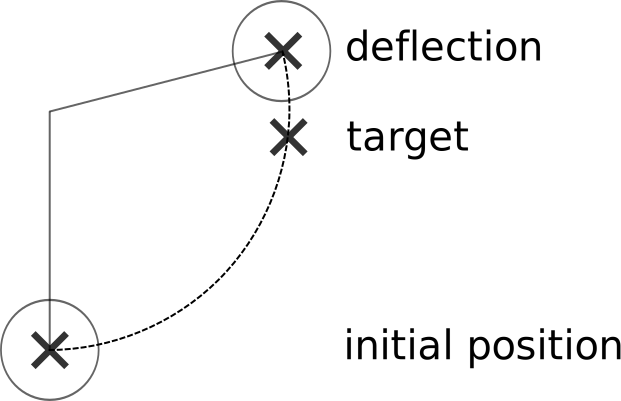
\includegraphics[width=0.45\textwidth]{pendulum}
\centering
\caption{
Pendulum deflection problem in xz-plane.
}
\label{fig:pendulum}
\end{figure}

Because there are many ways to not hit the pendulum at all, starting with
a high initial exploration will simplify the learning process. Therefore,
we set the initial step-size in Cartesian space to $500$ and in joint space
to $1250$.
The result is displayed in Figure \ref{fig:pendulum_res}. The advantage of
learning in Cartesian space almost vanishes in this environment. The
approximate inverse kinematic is slightly better than learning in joint
space but the exact inverse kinematic is worse. The reason for this becomes
obvious when we plot the reward surface in one dimension (see Figure
\ref{fig:pendulum_vary}).
The exact inverse kinematic has a very complex reward surface. There are
many local minima and abrupt changes of the reward. With the approximate
inverse kinematic the surface is a lot more smooth although there are still
local minima, however, CMA-ES can deal with these local minima when the
population size is large enough and the initial exploration is large enough.
The reward surface for learning in joint space is comparable to the
reward surface that corresponds to the approximate inverse kinematic.
Another observation that we can make is that there is a large flat
region in the reward surface where the end-effector does not hit the
pendulum. This region is much bigger for the joint space in this
dimension. Because the second weight belongs to the first joint of the
robot, it is possible that small modifications can easily steer the
end-effector in a completely different direction. CMA-ES automatically
learns the scaling of each dimension by adjusting the exploration
covariance, although this can take some updates.

\begin{figure}[tb]
\includegraphics[width=0.45\textwidth]{result_comparison_pendulum}
\centering
\caption{
Pendulum deflection results. The mean and standard error of the maximum reward
obtained so far is displayed.
}
\label{fig:pendulum_res}
\end{figure}

\begin{figure}[tb]
\includegraphics[width=0.45\textwidth]{vary_weight_pendulum}
\centering
\caption{
Projection of the reward surface of the pendulum problem on one axis.
To generate a projection of the reward surface on one DMP weight
dimension, we learned a DMP for 1000 episodes, kept the best policy,
modified the 2nd weight by adding an offset, and measured the
corresponding reward.
\todo[inline]{make this caption shorter}
}
\label{fig:pendulum_vary}
\end{figure}

\subsubsection{Pouring a Glass}

In this task, the robot fills a glass with marbles from a bottle while avoiding
nearby obstacles. The setup is displayed in Figure \ref{fig:pouring}. The
total number of marbles is 15.

The reward function is very complex.
For every marble that is inside of the glass, a reward of $1$ is given. For
every marble that is outside of the glass but on the table the negative
squared distance to the center of the glass is given. For every marble that
is still in the bottle we give a reward of $-1$. For collisions with
obstacles we give a reward of $-100$ and abort the episode. Marbles that
fall down the table also finish the episode and a reward of $-1000$ is
given.

\begin{figure}
\includegraphics[width=0.45\textwidth]{pouring}
\centering
\caption{
Pouring problem.
}
\label{fig:pouring}
\end{figure}

\todo[inline]{initial step-size? initial DMP?}

The results are displayed in Figure \ref{fig:pouring_res}.
Learning in joint space and learning in Cartesian space results in an
almost identical learning curve. Using an exact inverse kinematic
is again a lot worse than using an approximate solution.
The mapping from weights to reward in this problem is very complex,
nonlinear, and certainly not smooth. There are abrupt changes in
the reward function when a small change of one weight results in
a marble falling down the table or the arm touching an obstacle.
There are flat regions, for example, when all marbles stay
in the bottle because the arm does not turn the bottle upside down,
or all marbles miss the table. Therefore, the structure of the
reward surface is very complex independend of the space in which
we describe our DMPs, hence, learning in joint space and learning
in Cartesian space work similarly well.

\begin{figure}
\includegraphics[width=0.48\textwidth]{result_comparison_pouring}
\centering
\caption{
Pouring results. The mean and standard error of the maximum reward
obtained so far is displayed.
}
\label{fig:pouring_res}
\end{figure}

\subsection{Discussion}

\todo[inline]{Bitte korrekturlesen}

The artificial reinforcement learning problems that we presented vary in
the degree of indirection and smoothness of the reward function.

Weights in a DMP are bound to a specific radial basis function. As a result,
they only influence one dimension, that is, one specific joint or pose
dimension, and only have effects on the acceleration of the arm that are
local in time. That means they will affect the positions in all following
time steps but with a decreasing influence because the weight of the
learnable forcing term converges to zero.
So it is possible to design a reward function so that the optimization
problem becomes partially separable and, hence, very easy to solve.

For example, in the viapoint and obstacle avoidance problems we have an
almost direct relation between weights of the Cartesian DMP and the obtained
rewards (see Figure \ref{fig:mapping}).
With the approximate inverse kinematics we first use the weights to generate
a pose trajectory. This includes computing an acceleration based on the
linear forcing term that includes the weights and decays exponentially with
the time. The acceleration is integrated to obtain a trajectory of
end-effector poses. This trajectory might not be perfectly executable so that
in unreachable regions we have to map the pose to the closest reachable pose.
For the given viapoints we compute the distance to the corresponding poses
from the trajectory.
Hence, the mapping from specific weights to the reward in the workspace of
the robot is straightforward and the reward function becomes partially
separable.

In comparison to this very simple mapping, the joint space DMP results in a
much more complex mapping through the forward kinematics of the robot.
The mapping is nonlinear and increases coupling between the dimensions of
the weight space. This results in an optimization problem that is more
difficult because it is not partially separable any more with probably
multiple global and local optima.

The more complex the relation between weights and reward becomes, the
less significant is the difference between learning in joint space and
learning in Cartesian space.
The pendulum task is already a bit more complex because we cannot directly
relate the end-effector pose to the reward. Instead, the reward depends
nonlinearly on the momentum of the pendulum which depends on the position
and speed of the end-effector. The amount of nonlinearity and indirectness
almost renders the gained amount of directness by learning in Cartesian
space useless. Another difficulty of the problem is that the reward surface
is flat at most regions. If the end-effector does not hit the pendulum,
it will not move at all and the reward is -0.5.

The pouring problem is even more difficult. It has an almost flat reward
surface where the arm collides with an obstacle or a marble falls down.
Small weight changes can make the difference, for example, between a
marble staying within the glass and falling down, hence, the reward will
abruptly change in the corresponding regions of the weight space.
The relation between the DMP weights and a successful behavior is very
complex, highly nonlinear, and non-separable. This eradicates the
advantage of learning in Cartesian space.

\begin{figure}
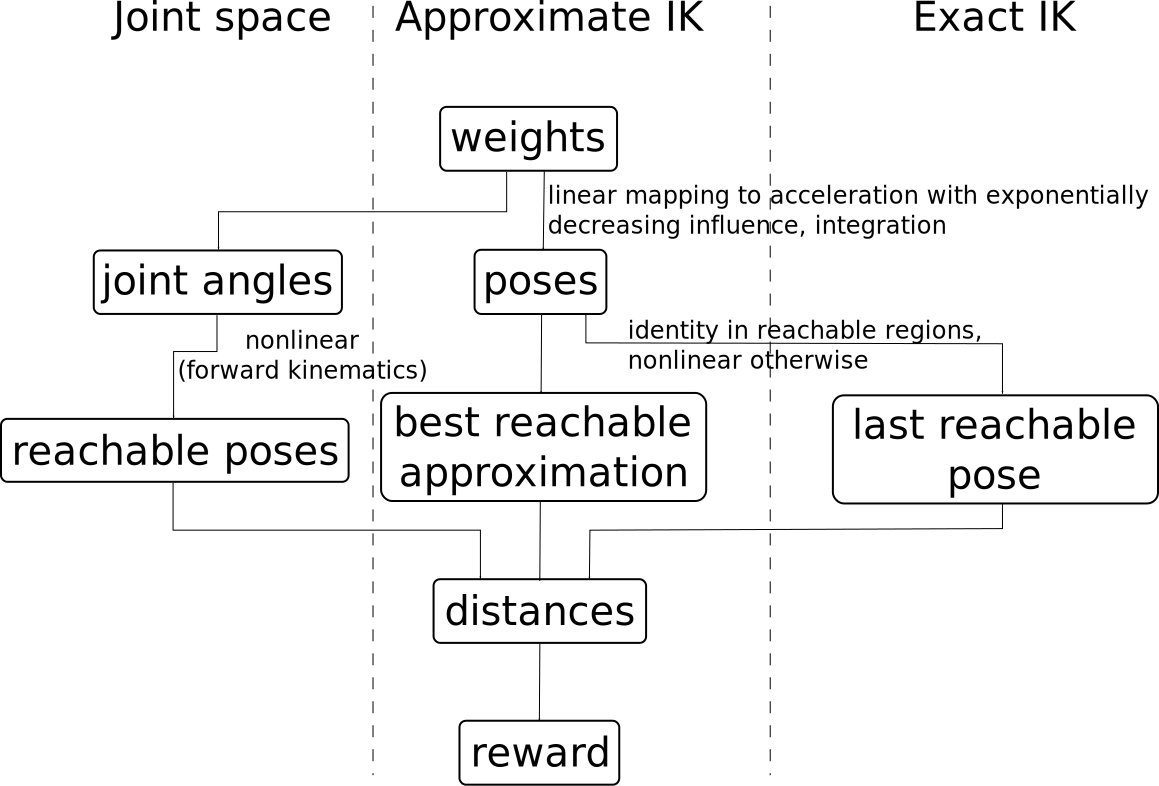
\includegraphics[width=0.45\textwidth]{mapping}
\centering
\caption{
Mapping from weights to corresponding reward in the viapoint problem.
For each setup different mappings are involved to compute the reward for
a weight vector.
}
\label{fig:mapping}
\end{figure}

\section{Conclusion}

Learning in Cartesian space is not always the best option.
It will be advantageous if the main objective has to be solved
Cartesian space and the reward function is almost separable.
It is not always obvious when this is the case though. For example, you would
probably think that target-directed ball-throwing with a robotic arm where
the target is given by its Cartesian position on the ground is a problem with
its main objective defined in Cartesian space.
We compared both learning in joint and in Cartesian space and the result was
that learning in joint space is much better. The reason for this is that the
inverse kinematic solutions did not result in trajectories that are as smooth
as it would be required to perform a good throwing motion.
Generating smooth trajectories is much simpler in joint space. Although policy
refinement in joint space works best for this problem, we can still use inverse
kinematics to transfer a demonstration that has been recorded in Cartesian
space (e.g. from a human) into the joint space of the robot to generate an
initial policy.

Hence, we could show that policy search works best in the space in which the
primary objectives are defined directly. We develop a configurable,
approximate variation of a state-of-the-art inverse kinematic solver and show
that it accelerates policy search for movement primitives in Cartesian space
in comparison to a conventional inverse kinematic solver. Using inverse
kinematics can be regarded as a way to include knowledge about the
kinematic structure of the target system in the learning process.

%\section*{Acknowledgments}

%This work was supported through two grants of the German Federal Ministry
%of Economics and Technology (BMWi, FKZ 50 RA 1216 and FKZ 50 RA 1217).

\appendix

%% The file named.bst is a bibliography style file for BibTeX 0.99c
\bibliographystyle{named}
\bibliography{literature}

\end{document}

